\documentclass[11pt,a4paper]{ctexart}
% Shared preamble for the assignment reports. Use with:
%   \documentclass[11pt,a4paper]{ctexart}  (XeLaTeX)
%   % Shared preamble for the assignment reports. Use with:
%   \documentclass[11pt,a4paper]{ctexart}  (XeLaTeX)
%   % Shared preamble for the assignment reports. Use with:
%   \documentclass[11pt,a4paper]{ctexart}  (XeLaTeX)
%   \input{../common/preamble.tex}
\usepackage[margin=2.3cm]{geometry}
\setmainfont{texgyretermes}[Extension=.otf,UprightFont=*-regular,BoldFont=*-bold,ItalicFont=*-italic,BoldItalicFont=*-bolditalic]
\setsansfont{texgyreheros}[Extension=.otf,UprightFont=*-regular,BoldFont=*-bold,ItalicFont=*-italic,BoldItalicFont=*-bolditalic]
\setmonofont{texgyrecursor}[Extension=.otf,UprightFont=*-regular,BoldFont=*-bold,ItalicFont=*-italic,BoldItalicFont=*-bolditalic]
\usepackage{amsmath,amssymb,mathtools,bm}
\usepackage{graphicx}
\usepackage{booktabs,multirow,makecell,array,tabularx}
\usepackage[table]{xcolor}
\usepackage[most]{tcolorbox}
\usepackage{enumitem}
\usepackage{listings}
\usepackage{subcaption}
\usepackage{siunitx}
\usepackage[hidelinks]{hyperref}
\usepackage[nameinlink,noabbrev]{cleveref}
\usepackage{float}

\setlength{\emergencystretch}{3em}
\linespread{1.15}
\setlist{leftmargin=*,itemsep=2pt,topsep=3pt}
\graphicspath{{figures/}}

\crefname{figure}{图}{图}
\crefname{table}{表}{表}
\crefname{section}{第}{第}
\creflabelformat{section}{#2#1#3 节}
\crefname{equation}{式}{式}
\crefformat{equation}{式~(#2#1#3)}

\lstset{basicstyle=\ttfamily\footnotesize,columns=fullflexible,breaklines=true,frame=single,
  framerule=0.3pt,rulecolor=\color{black!40},backgroundcolor=\color{black!3},
  keywordstyle=\color{blue!60!black}\bfseries,commentstyle=\color{green!40!black},
  numbers=left,numberstyle=\tiny\color{black!50},xleftmargin=1.5em}

% Interview boxes: question, model answer, common wrong answer.
\newtcolorbox{iqbox}[1]{enhanced,breakable,colback=blue!3,colframe=blue!45!black,boxrule=0.5pt,arc=1.5pt,
  left=4pt,right=4pt,top=3pt,bottom=3pt,fonttitle=\bfseries\small,title={面试追问：#1}}
\newtcolorbox{findingbox}[1][]{enhanced,breakable,colback=green!3,colframe=green!40!black,boxrule=0.5pt,arc=1.5pt,
  left=4pt,right=4pt,top=3pt,bottom=3pt,fonttitle=\bfseries\small,title={结论#1}}
\newtcolorbox{caveatbox}{enhanced,breakable,colback=orange!4,colframe=orange!60!black,boxrule=0.5pt,arc=1.5pt,
  left=4pt,right=4pt,top=3pt,bottom=3pt,fonttitle=\bfseries\small,title={不能推出的结论}}

\newcommand{\authorline}{ShaneLiu04\thanks{GitHub: \url{https://github.com/ShaneLiu04}。代码与原始指标见 edge-deploy 仓库各 lab 的 \texttt{artifacts/raw/}。本文基于公开课程材料独立完成，与课程团队无隶属关系。}}

\usepackage[margin=2.3cm]{geometry}
\setmainfont{texgyretermes}[Extension=.otf,UprightFont=*-regular,BoldFont=*-bold,ItalicFont=*-italic,BoldItalicFont=*-bolditalic]
\setsansfont{texgyreheros}[Extension=.otf,UprightFont=*-regular,BoldFont=*-bold,ItalicFont=*-italic,BoldItalicFont=*-bolditalic]
\setmonofont{texgyrecursor}[Extension=.otf,UprightFont=*-regular,BoldFont=*-bold,ItalicFont=*-italic,BoldItalicFont=*-bolditalic]
\usepackage{amsmath,amssymb,mathtools,bm}
\usepackage{graphicx}
\usepackage{booktabs,multirow,makecell,array,tabularx}
\usepackage[table]{xcolor}
\usepackage[most]{tcolorbox}
\usepackage{enumitem}
\usepackage{listings}
\usepackage{subcaption}
\usepackage{siunitx}
\usepackage[hidelinks]{hyperref}
\usepackage[nameinlink,noabbrev]{cleveref}
\usepackage{float}

\setlength{\emergencystretch}{3em}
\linespread{1.15}
\setlist{leftmargin=*,itemsep=2pt,topsep=3pt}
\graphicspath{{figures/}}

\crefname{figure}{图}{图}
\crefname{table}{表}{表}
\crefname{section}{第}{第}
\creflabelformat{section}{#2#1#3 节}
\crefname{equation}{式}{式}
\crefformat{equation}{式~(#2#1#3)}

\lstset{basicstyle=\ttfamily\footnotesize,columns=fullflexible,breaklines=true,frame=single,
  framerule=0.3pt,rulecolor=\color{black!40},backgroundcolor=\color{black!3},
  keywordstyle=\color{blue!60!black}\bfseries,commentstyle=\color{green!40!black},
  numbers=left,numberstyle=\tiny\color{black!50},xleftmargin=1.5em}

% Interview boxes: question, model answer, common wrong answer.
\newtcolorbox{iqbox}[1]{enhanced,breakable,colback=blue!3,colframe=blue!45!black,boxrule=0.5pt,arc=1.5pt,
  left=4pt,right=4pt,top=3pt,bottom=3pt,fonttitle=\bfseries\small,title={面试追问：#1}}
\newtcolorbox{findingbox}[1][]{enhanced,breakable,colback=green!3,colframe=green!40!black,boxrule=0.5pt,arc=1.5pt,
  left=4pt,right=4pt,top=3pt,bottom=3pt,fonttitle=\bfseries\small,title={结论#1}}
\newtcolorbox{caveatbox}{enhanced,breakable,colback=orange!4,colframe=orange!60!black,boxrule=0.5pt,arc=1.5pt,
  left=4pt,right=4pt,top=3pt,bottom=3pt,fonttitle=\bfseries\small,title={不能推出的结论}}

\newcommand{\authorline}{ShaneLiu04\thanks{GitHub: \url{https://github.com/ShaneLiu04}。代码与原始指标见 edge-deploy 仓库各 lab 的 \texttt{artifacts/raw/}。本文基于公开课程材料独立完成，与课程团队无隶属关系。}}

\usepackage[margin=2.3cm]{geometry}
\setmainfont{texgyretermes}[Extension=.otf,UprightFont=*-regular,BoldFont=*-bold,ItalicFont=*-italic,BoldItalicFont=*-bolditalic]
\setsansfont{texgyreheros}[Extension=.otf,UprightFont=*-regular,BoldFont=*-bold,ItalicFont=*-italic,BoldItalicFont=*-bolditalic]
\setmonofont{texgyrecursor}[Extension=.otf,UprightFont=*-regular,BoldFont=*-bold,ItalicFont=*-italic,BoldItalicFont=*-bolditalic]
\usepackage{amsmath,amssymb,mathtools,bm}
\usepackage{graphicx}
\usepackage{booktabs,multirow,makecell,array,tabularx}
\usepackage[table]{xcolor}
\usepackage[most]{tcolorbox}
\usepackage{enumitem}
\usepackage{listings}
\usepackage{subcaption}
\usepackage{siunitx}
\usepackage[hidelinks]{hyperref}
\usepackage[nameinlink,noabbrev]{cleveref}
\usepackage{float}

\setlength{\emergencystretch}{3em}
\linespread{1.15}
\setlist{leftmargin=*,itemsep=2pt,topsep=3pt}
\graphicspath{{figures/}}

\crefname{figure}{图}{图}
\crefname{table}{表}{表}
\crefname{section}{第}{第}
\creflabelformat{section}{#2#1#3 节}
\crefname{equation}{式}{式}
\crefformat{equation}{式~(#2#1#3)}

\lstset{basicstyle=\ttfamily\footnotesize,columns=fullflexible,breaklines=true,frame=single,
  framerule=0.3pt,rulecolor=\color{black!40},backgroundcolor=\color{black!3},
  keywordstyle=\color{blue!60!black}\bfseries,commentstyle=\color{green!40!black},
  numbers=left,numberstyle=\tiny\color{black!50},xleftmargin=1.5em}

% Interview boxes: question, model answer, common wrong answer.
\newtcolorbox{iqbox}[1]{enhanced,breakable,colback=blue!3,colframe=blue!45!black,boxrule=0.5pt,arc=1.5pt,
  left=4pt,right=4pt,top=3pt,bottom=3pt,fonttitle=\bfseries\small,title={面试追问：#1}}
\newtcolorbox{findingbox}[1][]{enhanced,breakable,colback=green!3,colframe=green!40!black,boxrule=0.5pt,arc=1.5pt,
  left=4pt,right=4pt,top=3pt,bottom=3pt,fonttitle=\bfseries\small,title={结论#1}}
\newtcolorbox{caveatbox}{enhanced,breakable,colback=orange!4,colframe=orange!60!black,boxrule=0.5pt,arc=1.5pt,
  left=4pt,right=4pt,top=3pt,bottom=3pt,fonttitle=\bfseries\small,title={不能推出的结论}}

\newcommand{\authorline}{ShaneLiu04\thanks{GitHub: \url{https://github.com/ShaneLiu04}。代码与原始指标见 edge-deploy 仓库各 lab 的 \texttt{artifacts/raw/}。本文基于公开课程材料独立完成，与课程团队无隶属关系。}}

\graphicspath{{../../solutions/mlc/e2e-relax/artifacts/figures/}}

\title{MLC 作业 1 实验报告：\\TVM 0.27 Relax 上的端到端 CNN——外部库、手写调度、MetaSchedule 与静默失效的调优数据库}
\author{\authorline}
\date{2026 年 11 月}

\begin{document}
\maketitle

\begin{abstract}
MLC 课程（陈天奇）作业 1 要求把 Fashion-MNIST 上训练好的 CNN 用 \path{BlockBuilder.emit_te} 搭成 Relax IRModule，把卷积换成外部库调用，再给卷积写调度~\cite{mlc,relax}。
本报告把作业从 2022 年的 TVM 迁移到 TVM 0.27~\cite{tvm}，在全部 10,000 张测试图上核对数值，额外跑 MetaSchedule~\cite{metaschedule}，并把端到端时间拆到每一层。
主要结论：
（a）五种 TVM 写法与 PyTorch 的准确率都是 83.88\%，最大绝对误差 $\le 4.2\times10^{-6}$，argmax 全部一致；
（b）默认编译每 batch 2375~µs，其中 linear0（$4\times100\times5408$）一层占 2344~µs，卷积只占 24~µs，只调卷积不改变端到端；
（c）给卷积和 linear0 都手写调度后 157~µs，MetaSchedule 640 次试验后 44~µs，PyTorch eager 505~µs；
（d）MetaSchedule 的数据库会静默失效：\path{tune_relax} 不融合、\path{compile_relax} 先融合再查表，两边的 PrimFunc 对不上，全部算子退回默认调度且不报错，第一次测得“调优后”2475~µs；
（e）TVM 线程池默认把线程绑到物理 CPU 0--7、无视 \texttt{taskset}，与其他任务共存时同一个并行 kernel 在 8~µs 与 620~µs 之间跳。
\end{abstract}

\section{设置}
网络：conv $3\times3$ 1$\to$32、ReLU、$2\times2$ max pool、flatten、linear 5408$\to$100、ReLU、linear 100$\to$10、softmax；权重是课程的 \texttt{fasionmnist\_mlp\_assignment\_params.pkl}，batch 4。
主机 Xeon Platinum 8470Q，\texttt{taskset} 限 8 核，PyTorch 2.8 单线程；TVM 的 target 与环境变量是
\begin{center}\small\texttt{llvm -mcpu=sapphirerapids -num-cores=8}，\quad \texttt{TVM\_NUM\_THREADS=8}，\quad \texttt{TVM\_BIND\_THREADS=0}。\end{center}
计时取 batch 4 一次调用的中位数：“VM 内”用 \texttt{time\_evaluator}，“Python 调用”另含 NumPy 与 TVM tensor 之间的两次拷贝。

\section{五种写法}
\textbf{emit\_te}：每个算子写一个 TE compute，权重以 \texttt{relax.const} 嵌入。
\textbf{外部库}：\path{tvm.register_global_func("env.conv2d")} 注册 NumPy 卷积，\texttt{relax.call\_dps\_packed} 调用，输出 buffer 由 Relax 分配（destination-passing style）。课程用 PyTorch 卷积；TVM 0.27 的 FFI 与 PyTorch 2.8 的 DLPack 扩展冲突，这里改用 NumPy。
\textbf{卷积调度}：输出通道按 4 切，$(n, f/4, y)$ 融合并行（832 个任务），$rc, ry, rx$ 居中，$f \bmod 4$ 展开，$x$（26）向量化；先标注再 \texttt{decompose\_reduction}，反过来做时 update block 没有 init、通不过向量化要求的 compact-dataflow 检查。
\textbf{linear0 调度}：$k$ 按 16 切后 \texttt{rfactor}，每条 lane 一个部分和，输出 $j$ 并行、lane 向量化。浮点归约不能原地向量化（会改变加法顺序），\texttt{rfactor} 把它显式改写成 16 路各自累加再合并。
\textbf{MetaSchedule}：\texttt{tune\_relax} 640 次试验、每批 32 个候选，604~s；builder 进程数取 \texttt{taskset} 的核数。

\begin{table}[H]
\centering\small
\caption{Fashion-MNIST 全部 10,000 张测试图，batch 4（\texttt{artifacts/raw/summary.json}）}\label{tab:main}
\begin{tabular}{lrrrr}
\toprule
写法 & 准确率 & 与 PyTorch 最大误差 & VM 内 µs & Python 调用 µs \\
\midrule
PyTorch eager（1 线程） & 83.88\% & — & — & 505 \\
Relax，默认编译 & 83.88\% & $4.2\times10^{-6}$ & 2375 & 2413 \\
Relax + 外部卷积（NumPy） & 83.88\% & $3.7\times10^{-6}$ & 4187 & 4239 \\
Relax，手写卷积调度 & 83.88\% & $4.2\times10^{-6}$ & 2578 & 2609 \\
Relax，手写卷积 + linear0 & 83.88\% & $2.0\times10^{-6}$ & 157 & 185 \\
Relax，MetaSchedule & 83.88\% & $4.2\times10^{-6}$ & \textbf{44} & \textbf{67} \\
\bottomrule
\end{tabular}
\end{table}

\begin{figure}[H]
\centering
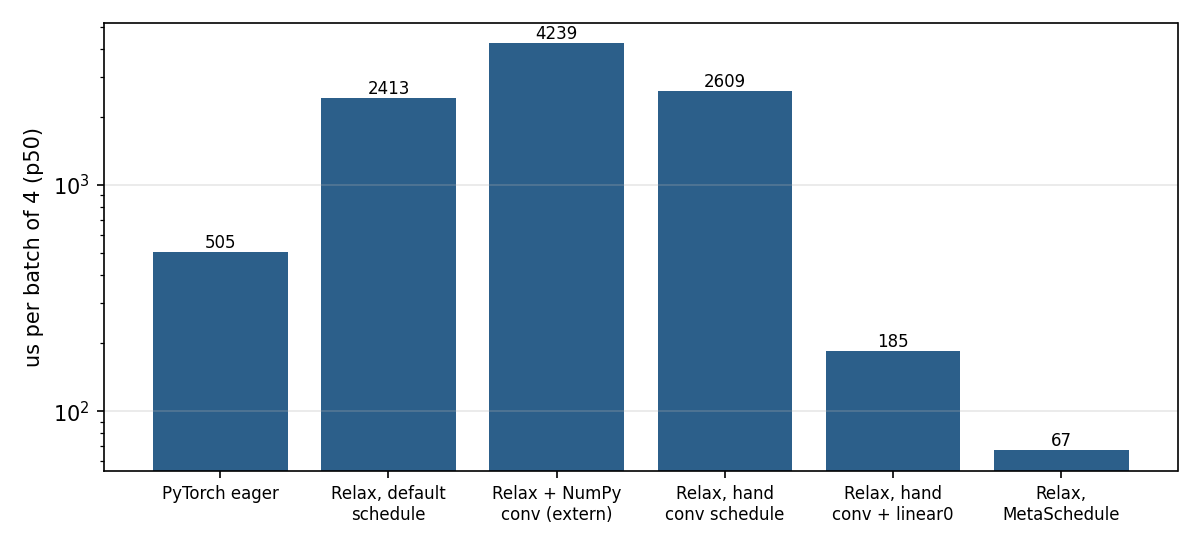
\includegraphics[width=0.9\linewidth]{e2e_latency.png}
\caption{每 batch 的 Python 调用时间（对数轴）。}\label{fig:lat}
\end{figure}

\section{时间花在哪里}
把网络的前 $k$ 层单独编译、计时（默认编译）：

\begin{table}[H]
\centering\small
\caption{默认编译下网络前 $k$ 层的 VM 时间（µs）}\label{tab:prefix}
\begin{tabular}{rrrrrrrrr}
\toprule
conv & +bias & +ReLU & +pool & +flatten & +linear0 & +ReLU & +linear1 & +softmax \\
\midrule
24 & 53 & 87 & 102 & 98 & 2442 & 2441 & 2379 & 2418 \\
\bottomrule
\end{tabular}
\end{table}

linear0 是 $4\times100\times5408 = 2.16$ M 次乘加，默认编译下是单线程标量循环（LLVM 不会在不允许重排加法的前提下向量化浮点归约），一层 2.3~ms；卷积只有 0.78 M 次乘加、内层是 26 宽的独立输出，LLVM 自动向量化后 24~µs。
所以作业要求的“给卷积写调度”在端到端上看不出来：手写卷积 kernel 单独计时从 21.4 降到 8.9~µs，但表~\ref{tab:main} 里那一行比默认编译还慢 200~µs，那是 linear0 那 2.3~ms 的波动（上一轮同样两种写法是 2417 对 2449~µs）。
给 linear0 加上 \texttt{rfactor} 调度后端到端降到 157~µs；剩下的主要是 bias、ReLU、pool 三个逐元素算子（合计约 80~µs，未调度、未融合）。
MetaSchedule 选出的六个融合 kernel 合计 32.9~µs，其中卷积 + bias + ReLU 5.0~µs、linear0 + ReLU 19.1~µs，融合省掉了逐元素算子的那部分。

\begin{iqbox}{小卷积为什么切得越细越慢？}
第一版调度把 $n, f, y, x$ 都切成 2--4 的小块、外层全部融合并行，每个任务只有十几次乘加，内层向量只有 4 宽；单独计时 53--60~µs，比朴素版的 21~µs 还慢。
改成“一行 26 个输出 $\times$ 4 个通道”为一个任务后 8.9~µs：每个任务足够大，能摊掉线程池的调度开销，内层仍是一整行向量。
\end{iqbox}

\section{两个静默失效}
\subsection{调优数据库对不上}
\texttt{compile\_relax} 先跑 \texttt{LegalizeOps}、\texttt{AnnotateTIROpPattern}、\texttt{FuseOps}、\texttt{FuseTIR}，再用 \texttt{MetaScheduleApplyDatabase} 按 PrimFunc 的结构查数据库；\texttt{tune\_relax} 抽任务时不跑融合。
直接调未融合的模块，数据库里是 9 个单算子（卷积 5.0~µs、linear0 19.1~µs 都调好了），编译时要查的是 6 个融合函数，一个都查不到，全部退回默认调度，端到端 2475~µs，与不调优相同，也没有任何警告。
反过来先融合、再把融合后的模块交给 \texttt{compile\_relax} 也不行：第二次 \texttt{AnnotateTIROpPattern} 给融合函数加上 \texttt{op\_pattern} 属性，结构哈希变了，最重要的两个函数（卷积、linear0）又查不到。
可用的组合是“调 \texttt{fuse(mod)}，编译 \texttt{mod}”，之后 6 个函数全部命中，端到端 44~µs。\texttt{tests/test\_relax.py} 把这一约束写成了测试：融合一次的函数没有 \texttt{op\_pattern}，融合两次的有。

\subsection{线程绑定无视 taskset}
默认 \texttt{TVM\_BIND\_THREADS=1} 时，TVM 线程池把工作线程按物理编号绑到 CPU 0--7，进程被 \texttt{taskset} 限在 8--15 也一样。MetaSchedule 在 0--7 上跑时，另一个进程里同一个并行卷积 kernel 三次运行分别是 8.9、619、7.3~µs；设 \texttt{TVM\_BIND\_THREADS=0} 后，七个调度变体两次运行最大相差 7~µs（52.6 对 59.8），不再出现百倍的跳变。

\begin{findingbox}[：MLC 作业 1]
端到端瓶颈是 linear0 而不是作业要求调度的卷积：默认编译 2375~µs 里它占 2344~µs，给它补一个 \texttt{rfactor} 调度就到 157~µs，MetaSchedule 到 44~µs；连同 Python 调用开销 67~µs，是 PyTorch eager（505~µs）的 7.5 分之一。
调优结果能不能用上，取决于调优与编译看到的 PrimFunc 是否逐结构相同，这一点 TVM 0.27 不检查也不报错；判断方法是逐层计时，而不是看调优日志里的最好延迟。
\end{findingbox}

\section{这些数字不能推出什么}
batch 4、$28\times28$ 的小网络里线程启动的固定开销占比高，换大 batch 或大模型各写法的比值会变。PyTorch 是 1 线程 eager、TVM 是 8 线程，这里比的是“编译器把这张网调到什么程度”，不是框架之间的公平对比。

\begin{thebibliography}{99}
\bibitem{mlc} T.~Chen, et~al. Machine Learning Compilation. \url{https://mlc.ai}, 2022.
\bibitem{tvm} T.~Chen, T.~Moreau, Z.~Jiang, L.~Zheng, E.~Yan, M.~Cowan, H.~Shen, L.~Wang, Y.~Hu, L.~Ceze, C.~Guestrin, A.~Krishnamurthy. TVM: An Automated End-to-End Optimizing Compiler for Deep Learning. \emph{OSDI}, 2018.
\bibitem{relax} R.~Lai, J.~Shao, S.~Feng, et~al. Relax: Composable Abstractions for End-to-End Dynamic Machine Learning. arXiv:2311.02103, 2023.
\bibitem{metaschedule} J.~Shao, X.~Zhou, S.~Feng, B.~Hou, R.~Lai, H.~Jin, W.~Lin, M.~Masuda, C.~H.~Yu, T.~Chen. Tensor Program Optimization with Probabilistic Programs. \emph{NeurIPS}, 2022.
\end{thebibliography}

\end{document}
